\documentclass{beamer}
\usetheme{Madrid}
\usecolortheme{default}

% --- 中文和数学包 ---
\usepackage[UTF8]{ctex}
\usepackage{amsmath, amssymb}
\usepackage{graphicx}
\usepackage{booktabs} % 用于更好看的表格
\usepackage{float}
\usepackage{subfigure}
\usepackage{algorithm}
\usepackage{algpseudocode}


% --- 定义一些常用命令 ---
\newcommand{\R}{\mathbb{R}}
\newcommand{\Lcal}{\mathcal{L}}
\newcommand{\Ncal}{\mathcal{N}}
\newcommand{\E}{\mathbb{E}}
\newcommand{\Var}{\mathrm{Var}}


%  % 中文默认字体：方正书宋_GBK（FZSSK.TTF），粗体为方正小标宋_GBK（FZXBSK.TTF），斜体为方正楷体_GBK(FZKTK.TTF)
% \setCJKmainfont { FZShuSong-Z01 }
%       [ BoldFont = FZXiaoBiaoSong-B05, ItalicFont = FZKai-Z03 ]
% % 中文无衬线字体：方正细黑一_GBK（FZXH1K.TTF），粗体为方正黑体_GBK（FZHTK.TTF）
% \setCJKsansfont { FZXiHeiI-Z08 } [ BoldFont = FZHei-B01 ]
% % 中文等宽字体：方正仿宋_GBK（FZFSK.TTF）
% \setCJKmonofont { FZFangSong-Z02 }

% % 中文字族
% \setCJKfamilyfont { zhsong } { FZShuSong-Z01  }
%       [ BoldFont = FZXiaoBiaoSong-B05 ]
% \setCJKfamilyfont { zhhei  } { FZHei-B01      }
% \setCJKfamilyfont { zhkai  } { FZKai-Z03      }
% \setCJKfamilyfont { zhfs   } { FZFangSong-Z02 }
% \setCJKfamilyfont { zhli   } { FZLiShu-S01    } % 方正隶书_GBK（FZLSK.TTF）
% \setCJKfamilyfont { zhyou  } { FZXiYuan-M01   } % 方正细圆_GBK（FZY1K.TTF），粗体为方正准圆_GBK（FZY3K.TTF）
%       [ BoldFont = FZZhunYuan-M02 ]


% --- 幻灯片信息 ---
\title[EviAdapt]{EviAdapt: 结合证据分位数回归的领域自适应 RUL 预测}
\subtitle{Evidential Domain Adaptation for Remaining Useful Life Prediction with Incomplete Degradation}
\author{汇报人：郭浩然}
\institute{ 西北工业大学 民航学院 }
\date{\today}


\begin{document}

% --- 标题页 ---
\begin{frame}
    \titlepage
\end{frame}

% --- 背景与动机 ---
\begin{frame}
    \frametitle{背景与动机}
    \begin{itemize}
        \item \textbf{核心任务：} 预测航空发动机的剩余使用寿命 (RUL) 

        \item \textbf{挑战1：领域偏移 (Domain Shift)}
        \begin{itemize}
            \item 训练与测试数据分布不一致 $\rightarrow$ 模型性能急剧下降。
            \item 主流解决方案：\textbf{领域自适应 (Domain Adaptation, DA)}。
        \end{itemize}

        \item \textbf{挑战2：目标域数据不完整}
        \begin{itemize}
            \item 真实场景中，设备很少被允许运行至完全失效。
            \item 导致目标域 (Target Domain) 严重缺乏“后期”退化数据。
        \end{itemize}
    \end{itemize}
\end{frame}

% --- 现有方法的局限性 ---
\begin{frame}[allowframebreaks]
    \frametitle{现有方法的局限性}
    \begin{columns}[T]
        \begin{column}{0.45\textwidth}
            \begin{block}{局限一：全局对齐导致阶段错配}
                \begin{itemize}
                    \item 传统DA方法试图对齐源域和目标域的\textbf{整体}特征分布。
                    \item 在目标域数据不完整时，会将目标域的“早期”退化阶段错误地与源域的“晚期”退化阶段对齐。
                    \item 后果：\alert{负迁移 (Negative Transfer)}。
                    \item 解决方式：将阶段进行划分后再进行对齐操作。
                \end{itemize}
            \end{block}
        \end{column}
        \begin{column}{0.45\textwidth}
            \begin{block}{局限二：同阶段特征模式不匹配}
                \begin{itemize}
                    \item 即使在相同的退化阶段，不同工况下的退化模式（如退化速率）也可能不同。
                    \item 导致特征表示 ($f_S, f_T$) 存在天然差异。
                    \item 解决方式：引入不确定性，对齐相应退化阶段之间的不确定性水平，而不是直接对齐特征
                \end{itemize}
            \end{block}
        \end{column}
    \end{columns}
    \begin{figure}[htbp] %H为当前位置，!htb为忽略美学标准，htbp为浮动图形
    \centering %图片居中
    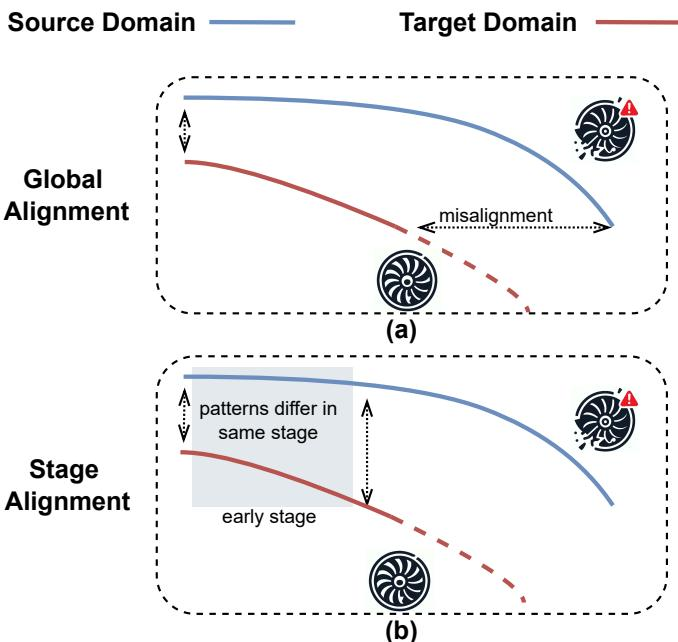
\includegraphics[width=0.5\textwidth]{./img/misalignment.jpg} %插入图片，[]中设置图片大小，{}中是图片文件名
    \caption{全局阶段对齐导致的阶段错配} %最终文档中希望显示的图片标题
    \label{misalignment} %用于文内引用的标签
    \end{figure}
\end{frame}

% --- 解决思路的演进 ---
\begin{frame}
    \frametitle{解决思路的演进与创新：从点估计到证据分位数回归}
    \begin{itemize}
        \item<1-> \textbf{传统回归 (MSE Loss):}
        \begin{itemize}
            \item 预测目标：因变量的期望 $E[y]$，输出一个\textbf{点估计}值。
            \item 缺点：无法表达预测的\alert{不确定性}。
        \end{itemize}
        \pause
        \item<2-> \textbf{引入不确定性 (Deep Evidential Regression, Amini et al. 2020):}
        \begin{itemize}
            \item 预测目标：为 $y$ 建模一个高阶证据分布 (Normal-Inverse-Gamma, NIG)。
            \item 模型输出NIG分布的四个参数 $(\gamma, \nu, \alpha, \beta)$，从中可解析出：
            $$ \underbrace{\mathbb{E}[\sigma^2] = \frac{\beta}{\alpha-1}}_{\text{偶然不确定性 (数据噪声)}} , \quad \underbrace{\mathrm{Var}[\mu] = \frac{\beta}{\nu(\alpha-1)}}_{\text{认知不确定性 (模型无知)}} $$
            \item \alert{局限：} 强依赖于“噪声服从高斯分布”的假设。
        \end{itemize}
        \pause
        \item<3-> \textbf{引入分位数回归 (Quantile Regression):}
        \begin{itemize}
            \item \textbf{目的：} 摆脱高斯分布假设，提供更灵活、鲁棒的分布描述。
            \item 预测目标：因变量的 $\tau$ 分位数，损失函数 $L_\tau(y, \hat{y})$ 非对称。
            \item \textbf{优势：} 通过预测多个分位数 (如Q25, Q75)，可描绘任意分布形态。
        \end{itemize}
        \pause
        \item<4-> \textbf{本文选择：融合两者优势 $\rightarrow$ \alert{证据贝叶斯分位数回归}}
    \end{itemize}
\end{frame}

% --- 方法详解1 ---
\begin{frame}[allowframebreaks]
    \frametitle{研究方法详解(1) - 核心技术与源域预训练}
    \begin{block}{核心技术：证据贝叶斯分位数回归}
        构建一个可以预测任意分位数 $q$ 及其不确定性的模型。
        \begin{itemize}
            \item 通过对正态分布的一个改造（引入$\tau = \frac{1 - 2q}{q(1 - q)}$ 和 $\omega = \frac{2}{q(1 - q)}$）$z \sim \mathrm{Exp}\left(\frac{1}{\beta / (\alpha - 1)}\right)$， $q$是手动规定的分位数），再套入Deep Evidential Regression的模型中,使得
            $$y_{S}\sim \mathcal{N}(\mu +\tau z,\omega \sigma^{2}z),\mu \sim \mathcal{N}(\gamma ,\sigma^{2}\nu^{-1}),\sigma^{2}\sim \Gamma^{-1}(\alpha ,\beta)$$
            \item 于是，$y_S$服从一个正态-逆伽马联合先验分布，即$$y_{S}\sim \mathcal{NIG}(\gamma, \nu, \alpha, \beta)$$
        \end{itemize}
    \end{block}
    
    \begin{block}{预训练阶段 (在源域)}
        \textbf{流程：} $f_S = E_S(X_S) \rightarrow (\gamma_S, \nu_S, \alpha_S, \beta_S) = R(f_S)$
        \vfill
        \textbf{损失函数：} $\Lcal_{total} = \sum_{q}(\Lcal_{NLL} + \lambda \Lcal_R)$
        \begin{itemize}
            \item $\Lcal_{NLL}$: Student-t 预测分布的负对数似然损失。
            $$ \Lcal_{NLL} = \frac{1}{2}\log(\frac{\pi}{\nu}) - \alpha\log(\dots) + (\alpha+\frac{1}{2})\log(\dots) + \dots $$
            \item $\Lcal_R$: 倾斜损失 (Tilted Loss)，作为正则项惩罚预测误差。
            $$ \Lcal_R = \max(q(y - \gamma), (q - 1)(y - \gamma))\Phi, \quad \text{where } \Phi = 2\nu + \alpha + 1 / \beta $$
        \end{itemize}
    \end{block}
\end{frame}

% --- 方法详解2 ---
\begin{frame}[allowframebreaks]
    \frametitle{方法详解(2) - 阶段分割与对齐}
    \begin{block}{第一步：阶段分割}
        \begin{itemize}
            \item \textbf{源域 (有标签):}
            \begin{itemize}
                \item 根据RUL标签和健康指数(HI)，划分为三阶段 (缓慢, 中等, 加速)。
            \end{itemize}
            \item \textbf{目标域 (无标签):}
            \begin{itemize}
                \item 使用预训练模型 ($E_S, R$) 生成\alert{伪标签}。
                \item 根据伪标签，划分为两阶段 (缓慢, 中等)。
                \end{itemize}
            \end{itemize}
        \end{block}
    \begin{block}{第二步：阶段化证据对齐}
        \begin{itemize}
            \item \textbf{核心思想：}
            不直接对齐特征 $f$, 而是对齐代表\alert{不确定性}的证据参数 $(\nu, \alpha, \beta)$。
            \item \textbf{对齐损失函数:}
            $$ \Lcal_{SEA} = -\sum_{n=1}^{2}\E[k((\nu_S, \alpha_S, \beta_S)_n, (\nu_T, \alpha_T, \beta_T)_n)] $$
            \item \textbf{解读：}
            \begin{itemize}
                \item $n=1, 2$ 代表缓慢和中等阶段。
                \item $k(\cdot, \cdot)$ 是核函数，衡量源域和目标域在\textbf{同一阶段}的\textbf{不确定性分布}的距离。
            \end{itemize}
        \end{itemize}
    \end{block}
    \vfill
    \begin{block}{训练过程}
        冻结预训练好的 $E_S, R$，仅优化目标编码器 \alert{$E_T$}, 使其能提取与源域对应阶段具有相似不确定性的特征。
    \end{block}
\end{frame}

\begin{frame}
    \frametitle{算法流程 (Part 3/3): 示意图}
    \begin{figure}[htbp] %H为当前位置，!htb为忽略美学标准，htbp为浮动图形
    \centering %图片居中
    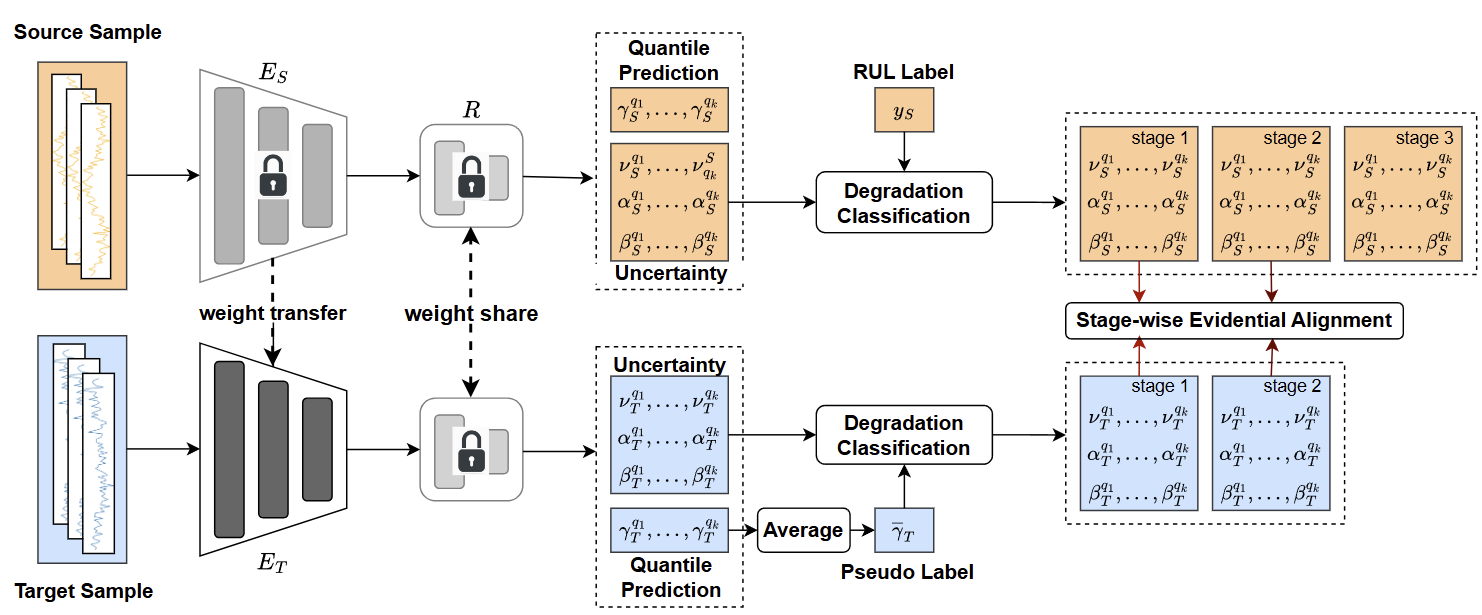
\includegraphics[width=\textwidth]{./img/image.png} %插入图片，[]中设置图片大小，{}中是图片文件名
    \caption{EviAdapt流程示意图} %最终文档中希望显示的图片标题
    \label{EviAdapt} %用于文内引用的标签
    \end{figure}
\end{frame}

% ===================================================================
%                 算法伪代码 (Part 1/2) - 手动拆分
% ===================================================================
\begin{frame}
    \frametitle{算法流程 (Part 1/3): 预训练与数据准备}
    
    \begin{algorithm}[H]
        \caption{EviAdapt: Pre-training and Staging}
        \begin{algorithmic}[1]
            \State \textbf{Input:} Source domain: $\{X_S, y_S\}$, Target domain: $X_T$
            \State \textbf{Output:} Trained target encoder $E_T$
            
            \State $E_S, R \gets \text{pretrain}(X_S, y_S)$ \Comment{在源域上预训练}
            \State $\gamma_T, \nu_T, \alpha_T, \beta_T \gets R(E_S(X_T))$ \Comment{为目标域生成证据参数}
            \State $\hat{y}_T \gets \text{average } \gamma_T \text{ over } [q_1, \dots, q_k]$ \Comment{生成伪标签}
            \State $X_{S1}, X_{S2}, X_{S3} \gets \text{stage segmentation for } X_S$ \Comment{源域阶段分割}
            \State $X_{T1}, X_{T2} \gets \text{stage segmentation for } X_T$ \Comment{目标域阶段分割}
            \State $\gamma_{S1}, \nu_{S1}, \dots \gets R(E_S(X_{S1}))$ \Comment{获取源域阶段1的证据}
            \State $\gamma_{S2}, \nu_{S2}, \dots \gets R(E_S(X_{S2}))$ \Comment{获取源域阶段2的证据}
        \end{algorithmic}
    \end{algorithm}
\end{frame}

% ===================================================================
%                 算法伪代码 (Part 2/2) - 手动拆分
% ===================================================================
\begin{frame}
    \frametitle{算法流程 (Part 2/3): 迭代对齐}
    \begin{algorithm}[H]
        \caption{EviAdapt: Iterative Alignment}
        \begin{algorithmic}[1]
             % 为了对齐行号，我们可以手动设置起始行号
            \setcounter{ALG@line}{7} % 从第8行开始
            
            \While{ iteration \textbf{do} }
                \State $\gamma_{T1}, \nu_{T1}, \dots \gets R(E_T(X_{T1}))$ \Comment{获取目标域阶段1的证据}
                \State $\gamma_{T2}, \nu_{T2}, \dots \gets R(E_T(X_{T2}))$ \Comment{获取目标域阶段2的证据}
                \State $loss \gets \mathcal{L}_{SEA}((\nu_S, \alpha_S, \beta_S)_n, (\nu_T, \alpha_T, \beta_T)_n)$ \Comment{计算对齐损失}
                \State $\theta_{E_T}^{(t+1)} = \theta_{E_T}^{(t)} - lr \cdot \nabla_{\theta_{E_T}} loss$ \Comment{更新目标编码器 $E_T$}
            \EndWhile
            
            \State \textbf{return} $E_T$
        \end{algorithmic}
    \end{algorithm}
\end{frame}



% --- 实验设置 ---
\begin{frame}
    \frametitle{实验设置}
    \begin{itemize}
        \item \textbf{数据集：}
        \begin{itemize}
            \item C-MAPSS, N-CMAPSS (航空发动机), PHM2010 (刀具磨损)。均为工业界公认基准。
        \end{itemize}
        \item \textbf{不完整场景模拟：}
        \begin{itemize}
            \item \alert{移除目标域训练集中后 40\% 的数据}，保留完整测试集。
        \end{itemize}
        \item \textbf{评价指标：}
        \begin{itemize}
            \item RMSE: 均方根误差。
            \item Score: 非对称评分，对“过晚”的预测给予更重惩罚，更贴合实际应用。
        \end{itemize}
        \item \textbf{对比方法 (Baselines):}
        \begin{itemize}
            \item Source Only (无适应), DDC, CORAL, ADARUL (传统DA), Cons DANN (为不完整数据设计的DA)。
        \end{itemize}
    \end{itemize}
\end{frame}


% --- 实验结果与分析 ---
\begin{frame}
    \frametitle{实验结果与分析}
    % \begin{columns}[T]
    %     \begin{column}{1\textwidth}
    %         % \begin{block}{主要结果 (SOTA Performance)}
    %         %     \begin{itemize}
    %         %         \item 在C-MAPSS, N-CMAPSS, PHM2010的大多数跨域任务上，EviAdapt 在RMSE和Score指标上均达到SOTA。
    %         %         \item \alert{尤其在Score指标上提升显著}，证明了其在规避灾难性晚期预测方面的价值。
    %         %         \item \textit{[此处展示核心结果表格的精简版或图表]}
    %         %     \end{itemize}
    %         % \end{block}
    %         % \begin{block}{消融实验 (Ablation Study)}
    %         %     \begin{itemize}
    %         %         \item \textbf{证明1:} 阶段化对齐 (S) \textgreater 全局对齐 (G)。
    %         %         \item \textbf{证明2:} 不确定性对齐 (Unc) \textgreater 特征对齐 (Fea)。
    %         %         \item \textbf{结论：} 模型的两个核心创新点都是有效且必要的。
    %         %     \end{itemize}
    %         % \end{block}
    %     \end{column}
    %     \begin{column}{0.4\textwidth}
    %         % \begin{block}{可视化分析 (t-SNE)}
    %         %     %% TODO: 替换 'tsne.jpg' 为图6的实际路径
    %         %     \includegraphics[width=\textwidth]{tsne.jpg}
    %         %     \caption{适配前 (上) vs. 适配后 (下)。EviAdapt有效拉近了源域和目标域的特征分布。}
    %         % \end{block}
    %     \end{column}
    % \end{columns}
    \begin{block}{主要结果 (SOTA Performance)}
        \begin{itemize}
            \item 在C-MAPSS, N-CMAPSS, PHM2010的大多数跨域任务上，EviAdapt 在RMSE和Score指标上均达到SOTA。
            \item \alert{尤其在Score指标上提升显著}，证明了其在规避灾难性晚期预测方面的价值。
        \end{itemize}
    \end{block}
    \begin{block}{消融实验 (Ablation Study)}
        \begin{itemize}
            \item \textbf{证明1:} 阶段化对齐 (S) \textgreater 全局对齐 (G)。
            \item \textbf{证明2:} 不确定性对齐 (Unc) \textgreater 特征对齐 (Fea)。
            \item \textbf{结论：} 模型的两个核心创新点都是有效且必要的。
        \end{itemize}
    \end{block}
\end{frame}


% ===================================================================
%            我的复现结果 - NCMAPSS (简化版，更推荐)
% ===================================================================
\begin{frame}
    \frametitle{我的复现结果 (1) - NCMAPSS 提炼}
    \begin{block}{主要结果}
        \begin{itemize}
            \item \textbf{在 `DS01` 作为源域时，复现效果优于论文：}
                \begin{itemize}
                    \item DS01 → DS02 (RMSE): \textbf{6.44} vs 9.23
                    \item DS01 → DS02 (Score): \textbf{946} vs 1515
                \end{itemize}
            \item \textbf{在 `DS02`/`DS03` 作为源域时，结果未能完全匹配论文：}
                 \begin{itemize}
                    \item DS02 → DS01 (RMSE): 14.12 vs \textbf{9.69}
                    \item DS03 → DS02 (RMSE): 6.63 vs \textbf{5.81} (但很接近)
                 \end{itemize}
            \item \textbf{结论：} 复现结果验证了方法的有效性，尤其是在特定数据分布 (`DS01`) 下展现了更优的潜力。结果的差异性表明模型对源域数据特性较为敏感。
        \end{itemize}
    \end{block}
    \begin{block}{待讨论的问题}
        \begin{itemize}
            \item 为何 `DS01` 作为源域时效果更好？可能是 `DS01` 的退化模式更具普适性，或者超参数恰好更适合这个设定。
            \item 如何提升在 `DS02`/`DS03` 上的表现？是否需要针对性地调整超参数或数据预处理？
        \end{itemize}
    \end{block}
\end{frame}



% --- 总结与未来工作 ---
\begin{frame}
    \frametitle{总结与未来工作}
    \begin{block}{本文贡献}
        \begin{enumerate}
            \item 提出了一种新颖的\textbf{阶段化对齐}策略，专门解决RUL预测中目标域数据不完整导致的阶段错配问题。
            \item 创造性地引入\textbf{证据不确定性对齐}，为领域自适应提供了一个比特征更鲁棒的对齐目标，有效容忍特征模式的差异。
            \item 在多个基准数据集上进行了广泛实验，验证了方法的优越性。
        \end{enumerate}
    \end{block}
\end{frame}

% --- 个人学习总结与待探讨问题 ---
\begin{frame}
    \frametitle{个人学习总结与待探讨问题}
    \begin{block}{我的收获与思考}
        \begin{itemize}
            \item 深入学习了从传统回归到贝叶斯方法到证据分位数回归的技术演进路线，理解了其动机和优势。
            \item 初步理解了不确定性（特别是认知不确定性）可以作为领域自适应中一个比特征更本质、更鲁棒的对齐目标。
            \item 通过阅读相关背景文献和代码，澄清了模型预训练和对齐训练的具体流程。
            \item 学习了阅读论文的基本方法
        \end{itemize}
    \end{block}
\end{frame}


\begin{frame}
    \frametitle{个人学习总结与待探讨问题}
    \begin{alertblock}{待探讨的问题}
        \begin{enumerate}
            \item \textbf{伪标签的鲁棒性：} 目标域的阶段划分完全依赖伪标签。若源-目标域差异过大导致伪标签质量差，整个策略是否会崩溃？有无更鲁棒的无监督阶段划分方法？
            \item \textbf{阶段划分的方法问题：} 论文中对阶段的定义是基于经验设定的固定百分比（源域0-33\%-85\%-100\%，目标域0-70\%-100\%）不同类型设备的退化过程可能截然不同，有的可能长期处于缓慢退化，然后突然加速；有的则可能退化过程较为线性。固定的阈值可能无法准确捕捉到这些变化的“拐点”
            \item \textbf{数据不完整可能有多样性：} 论文只模拟了“生命周期末端数据缺失”这一种情况，现实中的数据缺失可能是多种多样的，例如传感器故障，数据中随机出现一些缺失段，新设备刚投入使用，只有非常早期的健康数据
        \end{enumerate}
    \end{alertblock}
\end{frame}

% --- Q&A ---
\begin{frame}
    \frametitle{致谢 \& Q\&A}
    \vfill
    \centering
    \Huge \textbf{感谢您的聆听！}
    \vfill
    \Large 请多指正！
    \vfill
\end{frame}


\end{document}
